\begin{frame}{Linear Attention Is an RNN}
  \begin{columns}[T,onlytextwidth]
    \column{0.54\textwidth}
      \begin{itemize}\footnotesize\itemsep0.3em
        \item[\textcolor{red}{$\blacktriangleright$}] Causal softmax attention for token $t$ of one head, with $q_t, k_t, v_t \in \mathbb{R}^{d_h}$:
          \[ o_t = \frac{\sum_{i\leq t} \exp\!\big(q_t^\top k_i/\sqrt{d_h}\big)\, v_i}{\sum_{j\leq t} \exp\!\big(q_t^\top k_j/\sqrt{d_h}\big)}. \]
          Step $t$ reads all $t$ cached keys and values.
        \item[\textcolor{red}{$\blacktriangleright$}] Katharopoulos et al.\ use a kernel $\phi(q)^\top\phi(k)$ instead, where $\phi$ maps a vector to positive features. Then $\phi(q_t)$ moves out of both sums:
          \begin{gather*}
            S_t = S_{t-1} + \phi(k_t)\,v_t^\top, \qquad z_t = z_{t-1} + \phi(k_t),\\
            o_t = S_t^\top \phi(q_t) \,/\, z_t^\top \phi(q_t).
          \end{gather*}
          $S_t \in \mathbb{R}^{d_h\times d_h}$ sums the key-value outer products so far; $z_t \in \mathbb{R}^{d_h}$ sums the keys and normalises the read.
      \end{itemize}
    \column{0.44\textwidth}
      \begin{itemize}\footnotesize\itemsep0.4em
        \item[\textcolor{red}{$\blacktriangleright$}] The result is a recurrent network with a matrix state. Each step costs $O(d_h^2)$ time and memory for any $t$, and there is no KV cache. Training stays parallel, as cumulative sums over the known sequence.
        \item[\textcolor{red}{$\blacktriangleright$}] The paper's map is $\phi(x) = \mathrm{elu}(x) + 1$, with elu the exponential linear unit: positive, and unlike ReLU it keeps a gradient for $x < 0$. Exact softmax is out of reach, because the exponential kernel needs infinitely many features.
        \item[\textcolor{red}{$\blacktriangleright$}] CIFAR-10 generated pixel by pixel, after one week of training: 17.85 images/s against 0.004 for softmax attention (4,462$\times$) and 0.32 for softmax with a KV cache (over 50$\times$), at 3.40 against 3.47 bits/dim (negative log-likelihood in bits per pixel channel; lower is better).
      \end{itemize}
  \end{columns}
  \vspace{0.1em}
  {\scriptsize Katharopoulos et al., ``Transformers are RNNs: Fast Autoregressive Transformers with Linear Attention,'' ICML 2020, \href{https://arxiv.org/abs/2006.16236v3}{arXiv:2006.16236v3}, Section~3, Tables~2 and~4.}
\end{frame}

\begin{frame}{The State Is an Associative Memory}
  \begin{columns}[T,onlytextwidth]
    \column{0.50\textwidth}
      \begin{itemize}\footnotesize\itemsep0.3em
        \item[\textcolor{red}{$\blacktriangleright$}] Drop $\phi$ and the normaliser and store the transpose, as the delta-rule papers do. A write adds an outer product; a read multiplies by a query $q$:
          \[ S_t = S_{t-1} + v_t k_t^\top, \qquad S_t\, q = \sum_{i\leq t} v_i\,(k_i^\top q). \]
          Each stored value $v_i$ comes back weighted by the match $k_i^\top q$.
        \item[\textcolor{red}{$\blacktriangleright$}] \textbf{Example}, $d_h = 2$: store $v_1$ under $k_1 = (1,0)^\top$ and $v_2$ under $k_2 = (0,1)^\top$. Reading with $k_1$ returns $v_1$. A third pair under $k_3 = (1,1)^\top/\sqrt{2}$ turns that read into $v_1 + 0.71\,v_3$.
        \item[\textcolor{red}{$\blacktriangleright$}] At most $d_h$ keys can be orthogonal, so beyond $d_h$ pairs exact recall is impossible. With $d_h = 64$, linear attention errs from about 60 pairs.
        \item[\textcolor{red}{$\blacktriangleright$}] Writing $v_1'$ under $k_1$ again makes the read return $v_1 + v_1'$: the memory can neither forget nor overwrite.
      \end{itemize}
    \column{0.48\textwidth}
      \centering
      \vspace{0.3em}
      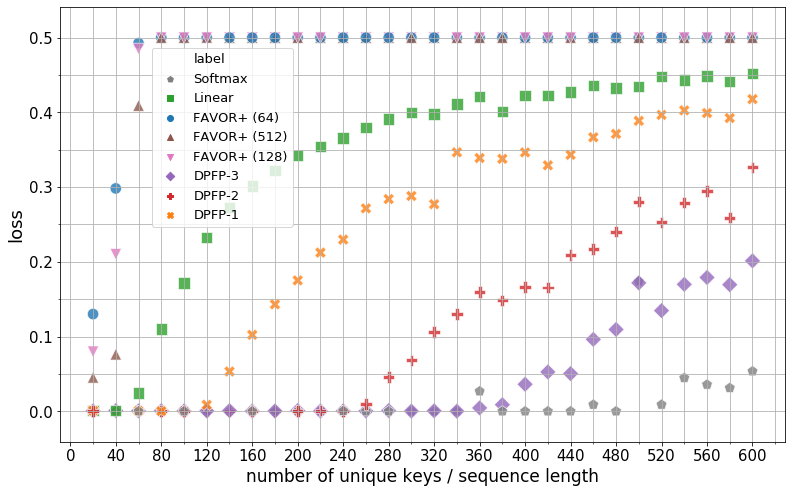
\includegraphics[width=\linewidth,height=0.52\textheight,keepaspectratio]{images/long-context/fwp_fig2_linear_attention_capacity.png}\\[0.2em]
      {\scriptsize Retrieval loss against the number of stored pairs, $d_h = 64$; green: linear attention, grey: softmax attention. Schlag et al., ``Linear Transformers Are Secretly Fast Weight Programmers,'' ICML 2021, \href{https://arxiv.org/abs/2102.11174v3}{arXiv:2102.11174v3}, Figure~2.}
  \end{columns}
\end{frame}

\begin{frame}{The Delta Rule Writes Only the Error}
  \begin{columns}[T,onlytextwidth]
    \column{0.54\textwidth}
      \begin{itemize}\footnotesize\itemsep0.3em
        \item[\textcolor{red}{$\blacktriangleright$}] Schlag et al.\ read the value stored under the incoming key, $\bar v_t = S_{t-1} k_t$, and replace it by the blend $\beta_t v_t + (1-\beta_t)\,\bar v_t$:
          \begin{align*}
            S_t &= S_{t-1} + \beta_t\,(v_t - S_{t-1}k_t)\,k_t^\top\\
                &= S_{t-1}\,(I - \beta_t k_t k_t^\top) + \beta_t\, v_t k_t^\top.
          \end{align*}
          $\beta_t \in (0,1)$ is a writing strength computed from the token. With unit-length keys, $\beta_t = 1$ replaces the old value exactly.
        \item[\textcolor{red}{$\blacktriangleright$}] Only the error $v_t - S_{t-1}k_t$ is written. The update is one gradient step, with learning rate $\beta_t$, on the loss $\tfrac{1}{2}\lVert S k_t - v_t\rVert^2$.
        \item[\textcolor{red}{$\blacktriangleright$}] The original algorithm ran token by token. Yang et al.\ made it chunkwise parallel and trained a 1.3B-parameter DeltaNet on 100B tokens.
      \end{itemize}
    \column{0.44\textwidth}
      \centering
      \vspace{0.4em}
      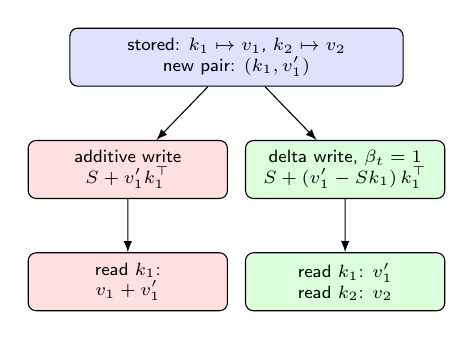
\begin{tikzpicture}[font=\sffamily\scriptsize, >=latex, scale=0.92,
          every node/.style={transform shape},
          box/.style={draw, rounded corners=0.1cm, align=center, minimum width=2.75cm, minimum height=0.8cm},
          mem/.style={box, fill=blue!12, minimum width=4.6cm},
          bad/.style={box, fill=red!12},
          good/.style={box, fill=green!14}]
        \node[mem] (m) at (0,3.1) {stored: $k_1 \mapsto v_1$,\ $k_2 \mapsto v_2$\\ new pair: $(k_1, v_1')$};
        \node[bad] (aw) at (-1.5,1.55) {additive write\\ $S + v_1' k_1^\top$};
        \node[good] (dw) at (1.5,1.55) {delta write, $\beta_t = 1$\\ $S + (v_1' - S k_1)\,k_1^\top$};
        \node[bad] (ar) at (-1.5,0) {read $k_1$:\\ $v_1 + v_1'$};
        \node[good] (dr) at (1.5,0) {read $k_1$: $v_1'$\\ read $k_2$: $v_2$};
        \draw[->] (m) -- (aw);
        \draw[->] (m) -- (dw);
        \draw[->] (aw) -- (ar);
        \draw[->] (dw) -- (dr);
      \end{tikzpicture}\\[0.4em]
      {\scriptsize The two-dimensional keys of the previous example. The delta write removes $v_1$ before adding $v_1'$. Since $k_2 \perp k_1$, neither write touches the pair under $k_2$.}
  \end{columns}
  \vspace{0.1em}
  {\scriptsize Schlag et al., \href{https://arxiv.org/abs/2102.11174v3}{arXiv:2102.11174v3}, Section~4.2; Yang et al., ``Parallelizing Linear Transformers with the Delta Rule over Sequence Length,'' NeurIPS 2024, \href{https://arxiv.org/abs/2406.06484v6}{arXiv:2406.06484v6}, Sections~2.2 and~3, Table~1.}
\end{frame}

\begin{frame}{Gated DeltaNet Adds a Decay Gate}
  \begin{itemize}\footnotesize\itemsep0.3em
    \item[\textcolor{red}{$\blacktriangleright$}] The delta rule edits one pair per step, so it cannot quickly clear the memory when the context changes. Mamba-2 can be written as linear attention with a scalar decay $\alpha_t$ that shrinks all pairs at once.
    \item[\textcolor{red}{$\blacktriangleright$}] Yang, Kautz \& Hatamizadeh combine the two in the \textbf{gated delta rule}, with $\alpha_t \in (0,1)$ computed from the token:
      \[ S_t = S_{t-1}\,\alpha_t\,(I - \beta_t k_t k_t^\top) + \beta_t\, v_t k_t^\top. \]
      $\alpha_t \to 0$ empties the memory, and $\alpha_t \to 1$ gives back the pure delta rule.
  \end{itemize}
  \vspace{0.1em}
  {\centering\scriptsize
  \begin{tabular}{p{2.4cm} p{5.2cm} p{2.0cm} p{2.0cm}}
    \toprule
    \textbf{Layer} & \textbf{State update} & \textbf{Forgets} & \textbf{Overwrites} \\
    \midrule
    Linear attention & $S_t = S_{t-1} + v_t k_t^\top$ & no & no \\
    Mamba-2 & $S_t = \alpha_t S_{t-1} + v_t k_t^\top$ & all pairs at once & no \\
    DeltaNet & $S_t = S_{t-1}(I - \beta_t k_t k_t^\top) + \beta_t v_t k_t^\top$ & no & the current key \\
    Gated DeltaNet & $S_t = S_{t-1}\,\alpha_t(I - \beta_t k_t k_t^\top) + \beta_t v_t k_t^\top$ & all pairs at once & the current key \\
    \bottomrule
  \end{tabular}\par}
  \vspace{0.2em}
  \begin{itemize}\footnotesize
    \item[\textcolor{red}{$\blacktriangleright$}] At 1.3B parameters and 100B training tokens each, WikiText perplexity is 16.42 for Gated DeltaNet, 16.56 for Mamba-2, 17.71 for DeltaNet and 18.53 for a Llama-style Transformer.
  \end{itemize}
  \vspace{0.1em}
  {\scriptsize Yang, Kautz \& Hatamizadeh, ``Gated Delta Networks: Improving Mamba2 with Delta Rule,'' ICLR 2025, \href{https://arxiv.org/abs/2412.06464v3}{arXiv:2412.06464v3}, Table~1 (update rules) and Table~3.}
\end{frame}

\begin{frame}{Infini-Attention: Local Attention Plus Memory}
  \begin{columns}[T,onlytextwidth]
    \column{0.56\textwidth}
      \begin{itemize}\footnotesize\itemsep0.3em
        \item[\textcolor{red}{$\blacktriangleright$}] Each layer splits its input into segments of $s = 2{,}048$ tokens and runs causal softmax attention inside each one, giving $a^{\text{dot}}_t$.
        \item[\textcolor{red}{$\blacktriangleright$}] The same queries, keys and values also use one linear-attention memory per head ($\phi = \mathrm{elu} + 1$). Segment $j$ reads what earlier segments wrote and is written when it ends:
          \[ a^{\text{mem}}_t = \frac{S_{j-1}\,\phi(q_t)}{z_{j-1}^\top \phi(q_t)}, \qquad S_j = S_{j-1} + \sum_{t \in j} v_t\, \phi(k_t)^\top. \]
          A delta variant writes $v_t$ minus the memory's current answer for $k_t$.
        \item[\textcolor{red}{$\blacktriangleright$}] A learned scalar per head mixes the two: $o_t = g\, a^{\text{mem}}_t + (1-g)\, a^{\text{dot}}_t$, with $g = \mathrm{sigmoid}(\gamma)$.
        \item[\textcolor{red}{$\blacktriangleright$}] The memory is $d_h^2 + d_h$ numbers per head and layer. Perplexity on PG19 books: 9.65, against 11.37 for Memorizing Transformers with a 114$\times$ larger memory. A 1B model fine-tuned on 5K-token inputs finds a passkey hidden in 1M tokens; an 8B model set the BookSum (book summarisation) record at 500K.
      \end{itemize}
    \column{0.42\textwidth}
      \centering
      \vspace{0.2em}
      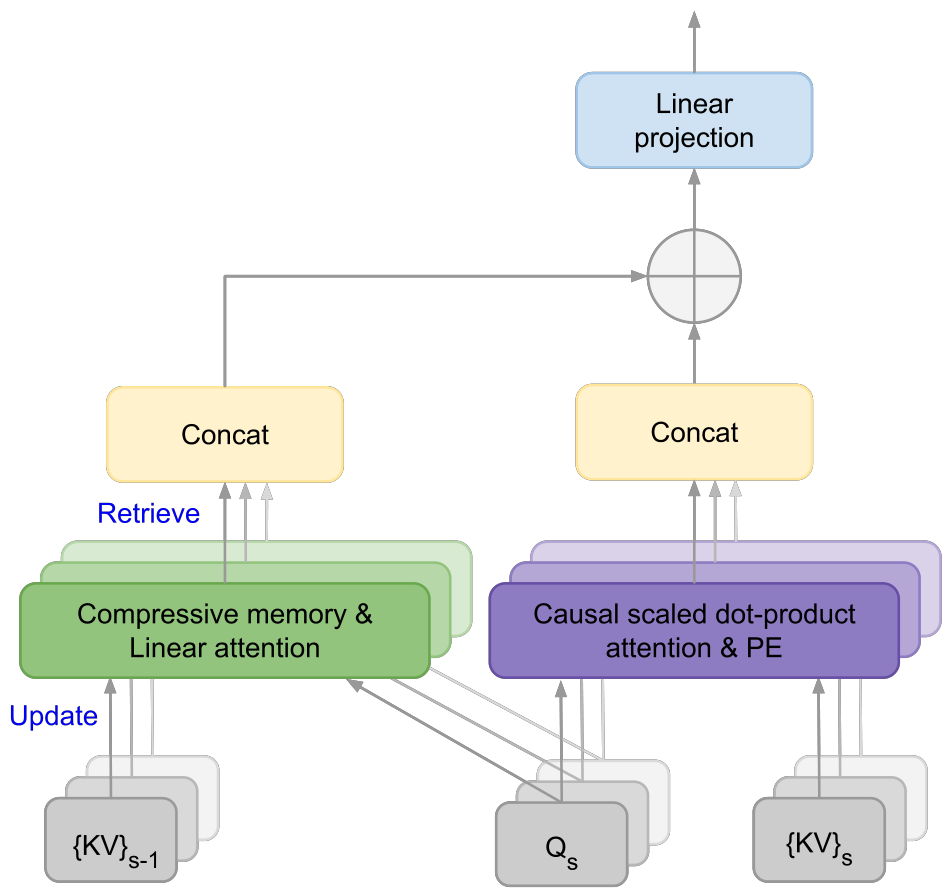
\includegraphics[width=\linewidth,height=0.58\textheight,keepaspectratio]{images/long-context/infini_attention_fig1_compressive_memory.png}\\[0.2em]
      {\scriptsize Munkhdalai et al., ``Leave No Context Behind: Efficient Infinite Context Transformers with Infini-attention,'' preprint 2024, \href{https://arxiv.org/abs/2404.07143v2}{arXiv:2404.07143v2}, Figure~1; numbers from Tables~1--4.}
  \end{columns}
\end{frame}

\begin{frame}{Titans: A Memory Trained at Test Time}
  \begin{columns}[T,onlytextwidth]
    \column{0.54\textwidth}
      \begin{itemize}\footnotesize\itemsep0.3em
        \item[\textcolor{red}{$\blacktriangleright$}] Behrouz et al.\ make the memory a small MLP $\mathcal{M}$, written by gradient steps on $\ell(\mathcal{M}_{t-1}; x_t) = \lVert \mathcal{M}_{t-1}(k_t) - v_t \rVert_2^2$. The gradient is the token's \textbf{surprise}. For a linear $\mathcal{M}$, one step is the delta rule.
        \item[\textcolor{red}{$\blacktriangleright$}] Surprise keeps momentum, and old content decays:
          \begin{gather*}
            u_t = \eta_t\, u_{t-1} - \theta_t\, \nabla \ell(\mathcal{M}_{t-1}; x_t),\\
            \mathcal{M}_t = (1-\alpha_t)\,\mathcal{M}_{t-1} + u_t.
          \end{gather*}
          The momentum decay $\eta_t$, step size $\theta_t$ and forget rate $\alpha_t \in [0,1]$ come from the token; $\alpha_t \to 1$ clears the memory, as $\alpha_t \to 0$ does in Gated DeltaNet. A read is a forward pass with no weight update.
        \item[\textcolor{red}{$\blacktriangleright$}] Memory as \textbf{context} prepends retrieved vectors and learned persistent tokens to each segment before attention; memory as a \textbf{gate} or a \textbf{layer} pairs it with sliding-window attention.
        \item[\textcolor{red}{$\blacktriangleright$}] Needle at 16K tokens (pass key / number / word): memory as context 98.4 / 97.4 / 95.2, DeltaNet 71.4 / 5.4 / 0.0, Mamba-2 5.4 / 0.0 / 0.0.
      \end{itemize}
    \column{0.44\textwidth}
      \centering
      \vspace{0.2em}
      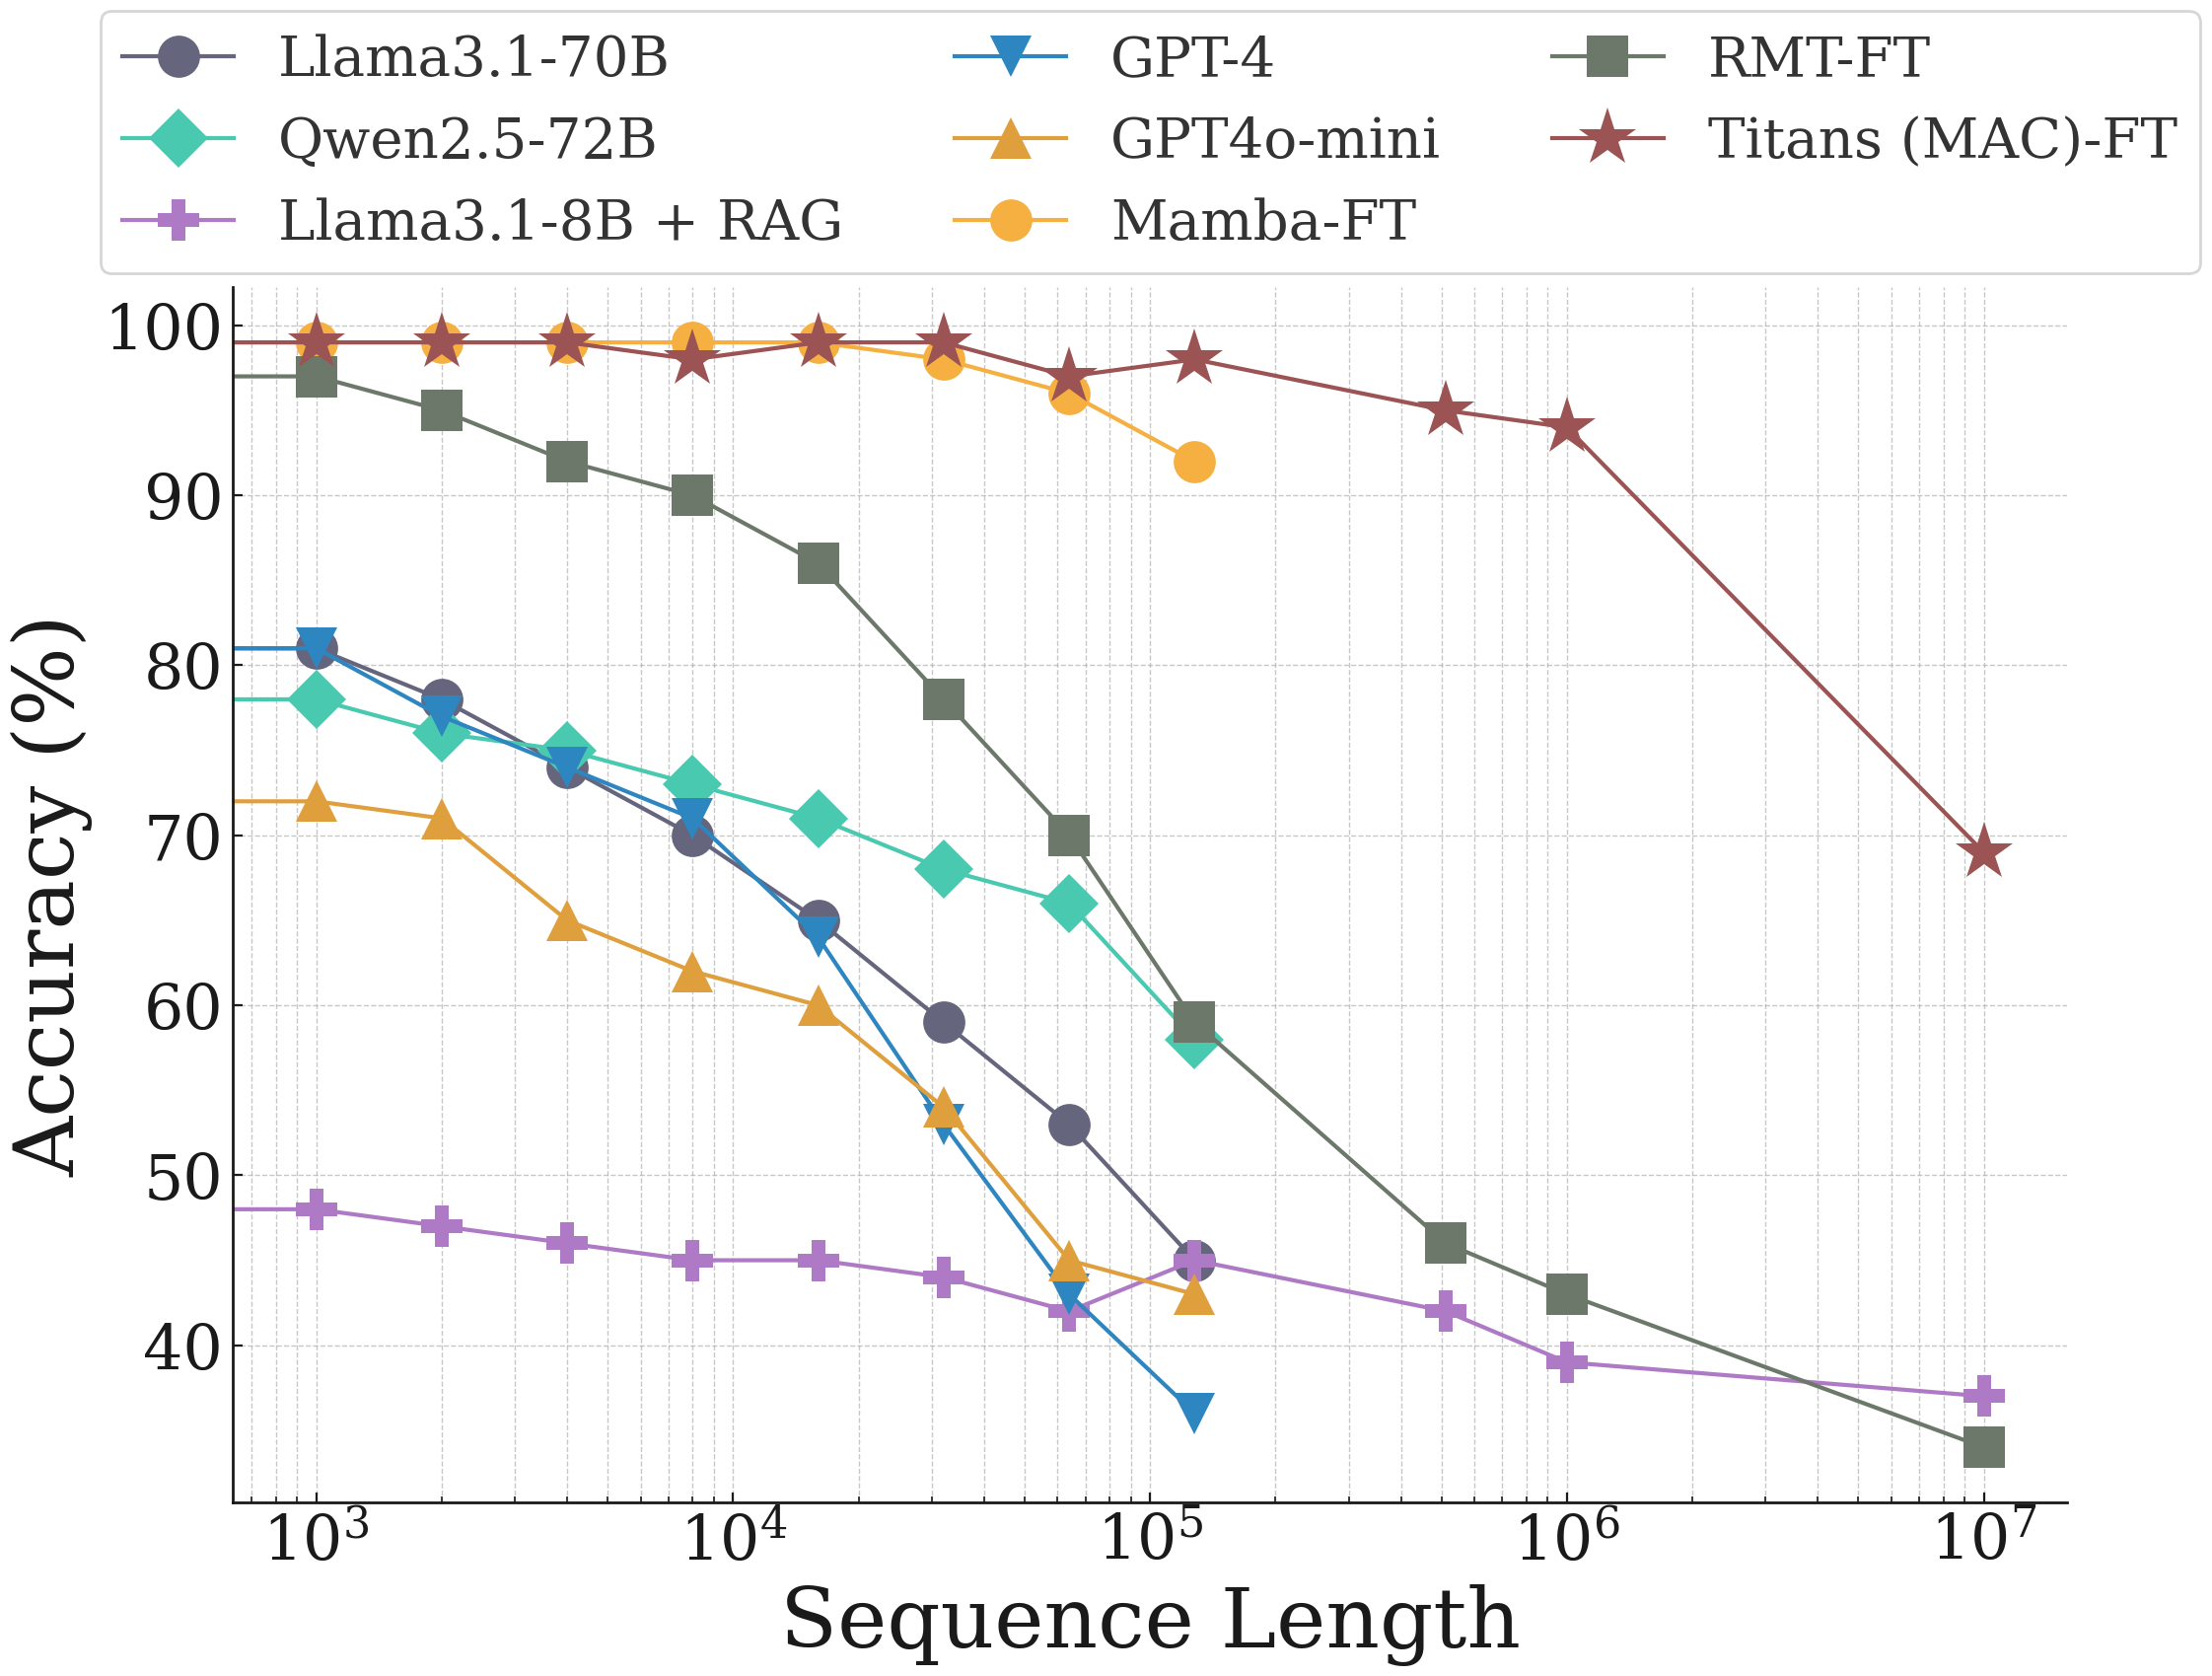
\includegraphics[width=\linewidth,height=0.52\textheight,keepaspectratio]{images/long-context/titans_fig6b_babilong_finetuned.png}\\[0.2em]
      {\scriptsize BABILong (questions about facts scattered through long texts), fine-tuned setting; red stars: Titans with memory as context. Behrouz et al., ``Titans: Learning to Memorize at Test Time,'' preprint 2024, \href{https://arxiv.org/abs/2501.00663v1}{arXiv:2501.00663v1}, Figure~6(b); needle scores from Table~2.}
  \end{columns}
\end{frame}

\begin{frame}{What a Fixed-Size Memory Costs}
  \begin{columns}[T,onlytextwidth]
    \column{0.52\textwidth}
      \begin{itemize}\footnotesize\itemsep0.3em
        \item[\textcolor{red}{$\blacktriangleright$}] Every memory in this section has a fixed size, so the copying result applies.
        \item[\textcolor{red}{$\blacktriangleright$}] \textbf{Recall-heavy tasks} (table): Gated DeltaNet trails the Transformer by 6.4 points on average and by 28.5 on FDA. Attention layers whose 2K window spans these inputs close the gap.
        \item[\textcolor{red}{$\blacktriangleright$}] \textbf{Needles:} trained on 4K tokens, Gated DeltaNet finds a number hidden in essays 100.0\% of the time at 1K tokens and 29.6\% at 8K.
        \item[\textcolor{red}{$\blacktriangleright$}] \textbf{At scale:} from 410M to 7B parameters, MiniMax's lightning attention (a linear attention) matched softmax on common-sense tasks but fell short at needle retrieval, so its production model keeps one softmax layer in eight.
        \item[\textcolor{red}{$\blacktriangleright$}] \textbf{Independent check:} Hugging Face could not make Infini-attention reliable; quality fell as the number of memory compressions grew.
      \end{itemize}
    \column{0.46\textwidth}
      \centering
      \vspace{0.2em}
      {\footnotesize Accuracy (\%), inputs truncated to 2K tokens}\\[0.3em]
      {\scriptsize
      \setlength{\tabcolsep}{3pt}
      \begin{tabular}{l c c c}
        \toprule
        \textbf{1.3B model} & \textbf{SWDE} & \textbf{FDA} & \textbf{Avg of 6} \\
        \midrule
        Mamba-2 & 19.1 & 25.3 & 29.8 \\
        DeltaNet & 17.9 & 18.4 & 26.2 \\
        Gated DeltaNet & 25.4 & 23.7 & 30.6 \\
        \addlinespace[0.15em]
        Llama-style Transformer & 29.5 & 52.2 & 37.0 \\
        Gated DeltaNet + SWA & 35.6 & 52.0 & 39.0 \\
        \bottomrule
      \end{tabular}\par}
      \vspace{0.4em}
      {\scriptsize SWA: sliding-window attention layers, 2K window. SWDE: extract relations from web pages. FDA: retrieve key-value pairs from PDF documents. All models trained on the same 100B tokens. Yang, Kautz \& Hatamizadeh, \href{https://arxiv.org/abs/2412.06464v3}{arXiv:2412.06464v3}, Table~4; needles from Table~2.}
  \end{columns}
  \vspace{0.2em}
  {\scriptsize MiniMax, ``MiniMax-01: Scaling Foundation Models with Lightning Attention,'' technical report 2025, \href{https://arxiv.org/abs/2501.08313v1}{arXiv:2501.08313v1}, Section~2.2 and Figure~7; Nguyen, von Werra \& Wolf, ``A Failed Experiment: Infini-Attention, and Why We Should Keep Trying?,'' Hugging Face blog, 14 Aug.\ 2024, \href{https://huggingface.co/blog/infini-attention}{huggingface.co/blog}.}
\end{frame}

\begin{frame}{Delta-Rule Hybrids in 2025 Models}
  \centering
  {\scriptsize
  \setlength{\tabcolsep}{4pt}
  \begin{tabular}{>{\raggedright\arraybackslash}p{2.0cm} >{\raggedright\arraybackslash}p{3.2cm} >{\raggedright\arraybackslash}p{3.1cm} >{\raggedright\arraybackslash}p{1.7cm} >{\raggedright\arraybackslash}p{2.3cm}}
    \toprule
    \textbf{Model} & \textbf{Linear layer} & \textbf{Full attention, ratio} & \textbf{Params (active)} & \textbf{Context} \\
    \midrule
    Qwen3-Next-80B-A3B, Sep.\ 2025 & Gated DeltaNet & softmax with a sigmoid output gate; 3 : 1, 48 layers & 80B (3B) & 262,144; about 1M with YaRN \\
    \addlinespace[0.2em]
    Kimi Linear, Oct.\ 2025 & Kimi Delta Attention (Gated DeltaNet, per-channel decay) & MLA, no positional encoding; 3 : 1 & 48B (3B) & 1M; KV cache up to 75\% smaller \\
    \addlinespace[0.2em]
    MiniMax-Text-01, Jan.\ 2025 & lightning attention: linear, no delta rule & softmax with GQA; 7 : 1, 80 layers & 456B (45.9B) & 1M training, 4M inference \\
    \bottomrule
  \end{tabular}\par}
  \raggedright
  \vspace{-0.3em}
  \begin{itemize}\footnotesize\itemsep0.1em
    \item[\textcolor{red}{$\blacktriangleright$}] Jamba keeps one attention layer in eight beside Mamba layers; Qwen3-Next and Kimi Linear keep one in four beside delta-rule memories.
    \item[\textcolor{red}{$\blacktriangleright$}] Kimi Linear at 1M tokens: 1.84\,ms per output token against 11.48\,ms for full MLA (over 6$\times$, helped by larger batches; 2.2$\times$ at batch size 1). Its ablation preferred 3:1 to 7:1, 15:1 or full attention alone.
    \item[\textcolor{red}{$\blacktriangleright$}] MiniMax returned to full attention for M2 (Oct.\ 2025): its hybrid had shown multi-hop reasoning deficits at scale, and other hidden weaknesses could not be ruled out.
  \end{itemize}
  {\scriptsize Qwen3-Next model card, \href{https://huggingface.co/Qwen/Qwen3-Next-80B-A3B-Instruct}{huggingface.co/Qwen}; Qiu et al., ``Gated Attention for Large Language Models: Non-linearity, Sparsity, and Attention-Sink-Free,'' preprint 2025, \href{https://arxiv.org/abs/2505.06708v1}{arXiv:2505.06708v1}; Kimi Team, ``Kimi Linear: An Expressive, Efficient Attention Architecture,'' technical report 2025, \href{https://arxiv.org/abs/2510.26692v2}{arXiv:2510.26692v2}; MiniMax, \href{https://arxiv.org/abs/2501.08313v1}{arXiv:2501.08313v1}; MiniMax, ``Why Did MiniMax M2 End Up as a Full Attention Model?,'' Hugging Face blog, 30 Oct.\ 2025, \href{https://huggingface.co/blog/MiniMax-AI/why-did-m2-end-up-as-a-full-attention-model}{huggingface.co/blog}.}
\end{frame}
